% 
% Annual Cognitive Science Conference
% Sample LaTeX Paper -- Proceedings Format
% 

% Original : Ashwin Ram (ashwin@cc.gatech.edu)       04/01/1994
% Modified : Johanna Moore (jmoore@cs.pitt.edu)      03/17/1995
% Modified : David Noelle (noelle@ucsd.edu)          03/15/1996
% Modified : Pat Langley (langley@cs.stanford.edu)   01/26/1997
% Latex2e corrections by Ramin Charles Nakisa        01/28/1997 
% Modified : Tina Eliassi-Rad (eliassi@cs.wisc.edu)  01/31/1998
% Modified : Trisha Yannuzzi (trisha@ircs.upenn.edu) 12/28/1999 (in process)
% Modified : Mary Ellen Foster (M.E.Foster@ed.ac.uk) 12/11/2000
% Modified : Ken Forbus                              01/23/2004
% Modified : Eli M. Silk (esilk@pitt.edu)            05/24/2005
% Modified : Niels Taatgen (taatgen@cmu.edu)         10/24/2006
% Modified : David Noelle (dnoelle@ucmerced.edu)     11/19/2014

%% Change "letterpaper" in the following line to "a4paper" if you must.

\documentclass[10pt,letterpaper]{article}

\usepackage{cogsci}
\usepackage{commath}
\usepackage{graphicx}
\usepackage{pslatex}
\usepackage{siunitx}
\usepackage{apacite}
\usepackage{xcolor}  % for \textcolor

\newcommand{\todo}[1]{\textbf{\textsc{\textcolor{blue}{(TODO\@: #1)}}}}

\title{A Spiking Independent Accumulator Model for Winner-Take-All}

\author{{\large \bf Jan Gosmann (jgosmann@uwaterloo.ca)} \\
  {\large \bf Aaron R.
Voelker (arvoelke@uwaterloo.ca)} \\
  {\large \bf Chris Eliasmith (celiasmith@uwaterloo.ca)} \\
  Centre for Theoretical Neuroscience, University of Waterloo \\
  Waterloo, ON, Canada N2L 3G1
}

\begin{document}

\maketitle

\begin{abstract}
The winner-take-all (WTA) mechanism is an important component of many cognitive models.
\todo{Flesh this out a bit}
Here we compare two biologically plausible, spiking neuron
implementations of different WTA mechanisms. 
We first provide a novel spiking implementation of the well-known leaky, competing accumulator (LCA) model, by mapping the dynamics onto a population-level representation.
We then propose a new two-layer spiking independent accumulator (IA) model, and compare its performance against the LCA network on a variety of WTA benchmarks.
Our findings suggest that while the LCA network can rapidly adapt to new winners, the IA network is better suited for stable decision making in the presence of noise.

\textbf{Keywords:} Neural Engineering Framework; Nengo; winner-take-all; 
decision making; mutual inhibition; neural competition; dynamical systems
\end{abstract}

\section{Introduction}

Winner-take-all (WTA) networks provide a mechanism that selects the largest value among a number of possible inputs.
More precisely, given a $d$-dimensional vector corresponding to the non-negative utility of $d$ different choices, the desired output is positive for the dimension with highest utility (i.e., the ``winner'') and zero for all others.
This mechanism is regularly employed as a component of cognitive models involving decision making, in which the action with the highest utility is selected to drive behaviour~\cite<e.g.,>{oreilly1998}. 
\todo{Cite survey or cite other examples}

A large body of literature exists examining the optimality of WTA mechanisms and their consistency with neurobiological and psychological data~\cite<e.g.,>{bogacz2006,gold2007,smith2004}.
Here, we investigate the suitability of two different WTA mechanisms in the context of large-scale cognitive modelling.
In particular, we map each mechanism onto a biologically plausible network of spiking neurons, and then compare them using a set of functional benchmarks that are normative in nature.
The first mechanism we consider is an implementation of the \emph{leaky, competing accumulator} (LCA) model from~\citeA{usher2001}.
The LCA model has been widely used, for example in versions of the Temporal Context Model~\cite{sederberg2008}, and in work on the Remote Associates Test \todo{not sure this is the right paper} models~\cite<e.g.,>{kajic2017}.
\todo{Add sentence somewhere differentiating our implementation from the latter implementation.  ce: only if it's fairly different}
The second mechanism we consider is the \emph{independent accumulator} (IA) model that we propose here, and which involves a secondary thresholding layer that is recurrently connected to a primary integrating layer.

For both mechanisms we are interested in decision-making tasks involving more than two choices ($d > 2$).
\todo{Misplaced sentence / unimportant here... ce: or flesh this out; can we say more about the nature of the tasks we're looking at... d>2 and d<10? what kind of speed do we want, etc?  or move this all later}

To implement each model, we use the Neural Engineering Framework~\cite<NEF;>{eliasmith2003} to map the model's dynamics onto populations of spiking neurons.
In the remainder of the paper, we provide a short introduction to the NEF, describe our implementation of the two WTA mechanisms, present our benchmarks, and finally discuss some resulting implications for cognitive modelling.

\section{Methods}

\subsection{The Neural Engineering Framework}
The Neural Engineering Framework~\cite<NEF;>{eliasmith2003} is a method of mapping a cognitive model, described using mathematical equations, onto a spiking neural network.
We now describe the aspects of this framework that are relevant to this work, by summarizing its three principles: \emph{representation}, \emph{transformation}, and \emph{dynamics}.

\subsubsection{Principle 1: Representation}
We define the representation of a scalar value $x(t)$ by an encoding and decoding with respect to some population of neurons.
The encoding of $x(t)$ into a spike train $a_i(t)$ for neuron $i$ is given by:
\begin{equation}
    a_i(t) = G_i\left[\alpha_i e_i x(t) + J_i^{\mathrm{bias}}\right] ,
\end{equation}
where $\alpha_i$ is a gain factor, $e_i$ is an encoder that determines a neuron's tuning curve, $J_i^{\mathrm{bias}}$ a bias current, and $G_i \left[ \cdot \right]$ is the neural nonlinearity.
Here, we use spiking, leaky integrate-and-fire (LIF) neurons for $G_i \left[ \cdot \right]$, and choose the encoders randomly.
Decoding weights $d_i$ are then used to approximate the represented value $\hat x(t)$ from the activity of the population of neurons by:
\begin{equation}
    \hat x(t) = \sum_i d_i \left[(a_i * h)(t)\right] ,
\end{equation}
where $h(t) = \tau_{\mathrm{s}}^{-1}\exp(t/\tau_{\mathrm{s}})$ is an exponentially decaying synaptic filter with time-constant $\tau_{\mathrm{s}}$, and $\ast$ is the convolution operator.
The decoding weights are obtained by least-squares optimization of the error $E_x = \abs{x - \hat{x}}$.
For the transmission of a value from one population to another, the connection weights are given by:
\begin{equation}
    W_{ij} = \alpha_j e_j d_i \text{.}
\end{equation}

\subsubsection{Principle 2: Transformation}
By finding alternate decoding weights $d^f_i$ with the error given by $E_{f(x)} = \abs{f(x) - \hat x}$, arbitrary linear and nonlinear functions $f(x)$ can be approximated in the connections between neural populations.

\subsubsection{Principle 3: Dynamics}
Given some nonlinear dynamics for the state variable $x(t)$:
\begin{equation} \label{eqn:nonlinear-system}
    \frac{\partial x}{\partial t} = g(x) ,
\end{equation}
we can map these dynamics onto a recurrent transformation, by harnessing the synaptic filter used in Principle 1.
In particular, for the exponentially decaying $h(t)$ we may apply Principle 2 to the recurrent transformation $f(x) = \tau_s g(x) + x$ to ensure that $x(t)$ obeys Equation~\ref{eqn:nonlinear-system}.

\subsection{Leaky, competing accumulator model}
Using the NEF, we have implemented the widely-used leaky, competing accumulator (LCA) model proposed by~\citeA{usher2001}.
The dynamics for each state variable $x_i(t),\ i < D$, where $D$ is the number of choices, are given by~(see Fig.~\ref{fig:usher-mcclelland}):
\begin{equation} \label{eqn:usher-mcclelland}
    \begin{split}
        \frac{{\partial x}_i}{\partial t} = \left(\rho_i - kx_i - \beta \sum_{j \neq i} x_j\right) \frac{1}{\tau}, \quad x_i &\ge 0,
    \end{split}
\end{equation}
where $\rho_i$ is each external input, $k$ is the leak rate, $\beta$ the lateral inhibition, and $\tau$ the time-constant.
This model essentially integrates each input $\rho_i$ with a leak term ($- kx_i$), minus competition from every other variable ($\beta \sum_{j \neq i} x_j$).
Supposing $\rho_i > \rho_j$ for all $j \ne i$, a WTA mechanism should indicate that $i$ is the winning choice.
Setting $k = \beta = 1$ will guarantee that the winning state $x_i$ converges to the value of the largest input $\rho_i$, while the losing states $x_j$ ($j \ne i$) converge to zero.
Other choices of $k$ merely alter the effective $\tau$ and the effective gain on the input, while other choices of $\beta$ will produce unwanted behaviour (see supplementary analysis).

We implement Equation~\ref{eqn:usher-mcclelland} with the NEF by using one population of neurons for each $x_i$, and applying Principle~3 to each population.
By appropriately selecting the gain and bias parameters from Principle~1, we ensure that each state variable is rectified ($x_i \ge 0$) as required.
We believe this implementation is novel as it does not interpret each $x_i$ as a distinct neural firing rate, but rather as a population-level representation distributed across any number of spiking neurons.
In effect, heterogeneous spike trains are weighted by optimal decoding weights to precisely implement the stated dynamics.
%As such, the model equations do not impose restrictions on the neuron model or requires to lump the neurons into a single population firing rate.
This allows us to attain greater biological realism without altering the dynamics prescribed by Equation~\ref{eqn:usher-mcclelland}.
\todo{distributing the states across neurons would be yet another implementation; maybe worth mentioning in the discussion...as that might be even more bio-plausible}

\begin{figure}
    \centering
    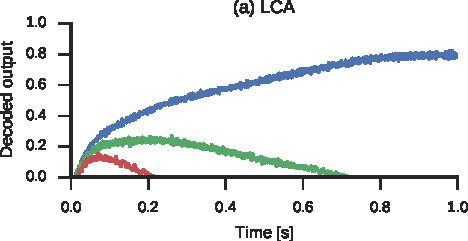
\includegraphics{figures/usher-mcclelland}
    \caption{
        Example time course of the state variables in the LCA network with three choices.
        The vector of inputs is given by $(0.8, 0.7, 0.6)$.
    }\label{fig:usher-mcclelland}
\end{figure}

\subsection{Independent accumulator model}
The other WTA mechanism that we investigate is our proposed independent accumulator (IA) model.
We use the term `independent' to refer to the fact that there are no direct interactions between each accumulator, unlike in the LCA model which has direct competition between states.
To enable a form of competition, we add a second thresholding layer that  projects back to self-excite and mutually-inhibit the first layer.
We now provide the details of each layer, again implemented with the principles of the NEF\@.
\todo{Network diagram?}

The first layer consists of a separate integrator population (i.e., accumulator) for each state variable $x_i(t), \ i < D$.
The second layer consists of independent, non-recurrent populations that receive input from the first layer in a one-to-one fashion.
From the second layer, we decode the function $\bar{x}_i := \Theta(x_i - \vartheta)$ where $\Theta$ is the Heaviside function, and $\vartheta = 0.8$ is a fixed threshold value that determines how much evidence needs to be accumulated to produce an output.
The Heaviside decoded output of layer 2 projects back to layer 1 to add $\bar{x}_i - \bar{\beta} \sum_{j \neq i} \bar{x}_j$ to the input of $x_i$.
Since intuitively the largest input will accumulate the fastest, once this reaches the threshold $\vartheta$ it will self-excite and inhibit all other state variables.
Fixing $\bar{\beta} = 2$ ensures that the losing state variables will go to zero (see supplementary analysis).
This is summarized more precisely by the following dynamics (see Fig.~\ref{fig:indacc}):
\begin{equation}
    \begin{split}
        \frac{{\partial x}_i}{\partial t} = \rho_i \frac{1}{\tau_1} + \left( 
            \bar{x}_i - \bar{\beta} \sum_{j \neq i} \bar{x}_j \right) \frac{1}{\tau_2} , \quad x_i &\ge 0 .
    \end{split}
\end{equation}
% should we say anything about how the thresholding population works?

%Instead of controlling the threshold $\vartheta$, it is more convenient to keep $\vartheta$ fixed and scale the input with the $\lambda$ parameter -- mathematically this is equivalent.
% ^ this isn't quite equivalent. you also need to multiply the Heaviside by lambda in order to keep the feedback having the same relative magnitude
% it would be equivalent to scale \tau_1 inversely with \lambda
% also I think this point isn't too important?
%As the LCA model does not have a threshold parameter, we do not introduce the input scaling $\lambda$ in that model.
\begin{figure}
    \centering
    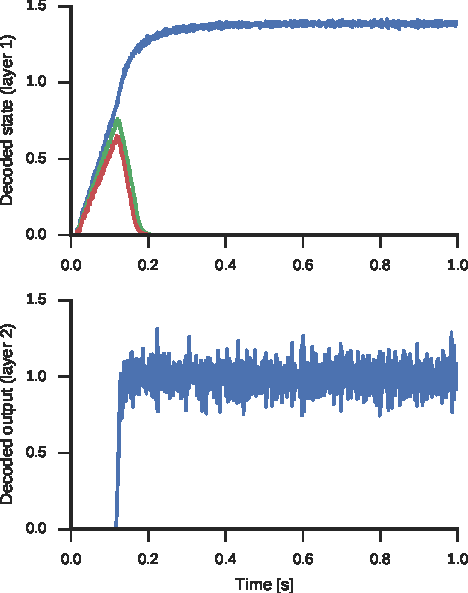
\includegraphics{figures/indacc}
    \caption{
        Example time course of the state variables $x_i$ and decoded output $\bar{x}_i$ in the IA network with three choices.
        The vector of inputs is given by (0.8, 0.7, 0.6).
        \todo{Put next to (or below) first figure.}
    }\label{fig:indacc}
\end{figure}

\subsection{Benchmarks}
To test and compare the two WTA mechanisms we provide an input of $\rho_i = u - s(1 - \delta_{1i}) + \eta_i$, where $u$ is the strength of the strongest input, 
$s > 0$ is the target separation relative to all other inputs, $\delta$ is the Kronecker delta, and $\eta_i$ is Gaussian (white) noise with standard deviation $\sigma$.
Thus, without loss of generality, the first state variable receives the strongest input $u$ plus noise, and all other state variables receive a noisy input that is smaller by $s$.
Since all of the runner-ups have equal magnitude, this represents the most difficult scenario of the network's capability where all potential choices must be considered.
As $s \rightarrow 0$ the problem becomes more difficult because the utilities of the choices are closer together.
We will use $u = 1$ unless indicated otherwise, and set the number of choices to $D = 10$.
Further, we chose noise variance increments large enough to observe how the networks start to fail performing their task.
In both WTA models we use 200 neurons per choice.
In the IA network this is split into 150 neurons for each layer 1 population and 50 neurons for each layer 2 population.
All remaining network parameters are summarized in Table~\ref{tbl:params}.
\begin{table}
    \caption{Summary of parameter values.}\label{tbl:params}
    \begin{tabular}{ll}
        LCA time-constant & $\tau = \SI{0.1}{\second}$ \\
        LCA recurrent parameters & $k = \beta = 1$ \\
        IA accumulation time-constant & $\tau_1 = \SI{0.1}{\second}$ \\
        IA feedback time-constant & $\tau_2 = \SI{0.1}{\second}$ \\
        IA threshold & $\vartheta = 0.8$ \\
        IA recurrent parameters & $\lambda = 1, \bar{\beta} = 2$ \\
        Recurrent synaptic time-constant & $\tau_{\mathrm{s}} 
        = \SI{0.1}{\second}$ \\
        Feed-forward synaptic time-constant & $\tau_{\mathrm{s}} 
        = \SI{0.005}{\second}$ \\
        Output decoding synaptic time-constant & $\tau_{\mathrm{s}} 
        = \SI{0.01}{\second}$
    \end{tabular}
\end{table}

To evaluate the two mechanisms on the previously defined input, we use a number of separate metrics.
First, we determine whether the model is able to form a clear decision within one second.
To be counted as `clear', at least one output must remain above 0.15 across the time interval $(\SI{1}{\second}, \SI{2}{\second}]$. % chktex 9
This lower bound of 0.15 was chosen to ensure that noise on a zero output is not mistaken for a non-zero output.
Note that this metric requires that the decision does not change throughout the time interval.
This does not take into account whether the winning output actually corresponds to the strongest input, but for some models it is more desirable to produce a clear incorrect decision than an unstable incorrect decision.
In other situations, though, the correctness of the decision may be of higher importance.
Thus, we consider a trial `correct' if the model forms a clear decision, and the largest output corresponds to the true largest input.

We now describe a number of metrics that will be calculated on the subset of trials that contain a clear decision.
% The time it takes to form a decision can be relevant too.
It is important to consider the speed at which the network can make decisions.
We therefore define the `decision time' as the length of time it takes to fulfil the conditions of a clear decision.
%These metrics cover the basic performance of the WTA mechanisms.
Likewise, when using a WTA mechanism within larger cognitive models, the exact magnitude of the outputs can be important.
Ideally, the output would be one for the winner and zero for all other outputs.\footnote{Technically, the winner output could be scaled to any magnitude.
We use $1$ for convenience.}
\todo{Have you tried decoding a threshold (say $\Theta(x_i - 0.15)$) off the LCA network?}
The LCA dynamics, however, prescribe an output of $u$ for the winner, with $u$ being the largest input.
We define the `winner error' $E_1$ as the difference of the winner output from $u$ for the LCA network, as the difference from one for the IA network and, for both models, the `runner-up error' $E_2$ as the difference of second largest output from zero (with negative values treated as zero).
We use the average output values over the time interval $(\SI{1}{\second}, \SI{2}{\second}]$ to calculate these error values (since these values fluctuate over time).  % chktex 9
These two metrics only consider the final output averaged over time, but the model can produce transient outputs before the final decision is achieved.
Within the context of a larger model, this can be a problem as the transient output could be prematurely interpreted as a decision.
Thus, we define $E_{2,\max}$ as the `highest output of a losing choice' during the whole simulation.

\section{Results}
We find that the ability to reach a clear decision depends on the magnitude of the highest input for both networks.
This is not surprising.
In the LCA network the output magnitude will be determined by the input magnitude of the largest input.
As such the largest input needs to be above 0.15 to fulfil the requirements.
For the IA network, the input has to be large enough to reach the integration threshold within the time limit.
By increasing the input scaling $\lambda$, or the time limit, one could get a clear decision for smaller inputs within the time limit.
We further find that the IA network is independent of the input noise and target separation for all tested parameters.\todo{but how does it do? can you put a single line on figure 3 to show it, so we can see the comparison to LCA? something visual would be good.}
This is not the case for the LCA network where the fraction of trials without a clear decision increases with noise and smaller target separation (see Fig.~\ref{fig:decisions}).
\begin{figure}
    \centering
    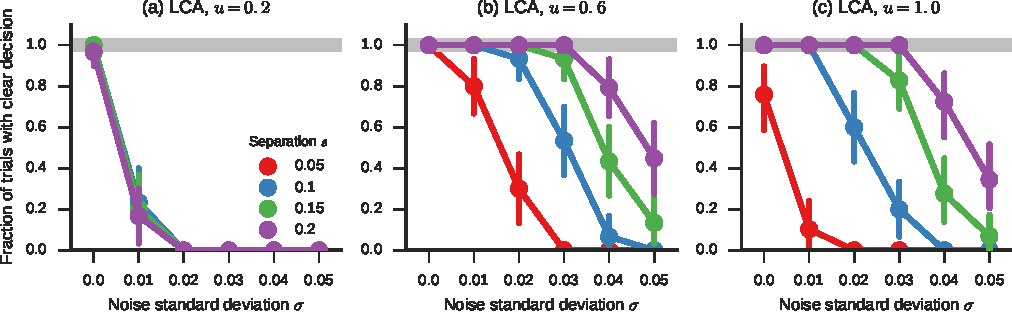
\includegraphics{figures/decisions}
    \caption{
        Fraction of trials with a clear decision for different input noise standard deviations $\sigma$ and target separations $s$ for the LCA network.
        Error bars denote bootstrapped 95\% confidence intervals.
        The grey horizontal line shows the optimum.
    }\label{fig:decisions}
\end{figure}

However, when considering the correctness of the decisions (see Fig.~\ref{fig:correct}) the LCA network does better with the default parameters.
We can alleviate that difference to some degree by reducing the input scaling to $\lambda = 0.2$, but the IA network still performs worse for some combinations of input noise and target separation when staying below the time limit.
This is part due in part to a systematic bias for certain choices introduced in the second layer of the IA network.
In the NEF the neuron gain and bias parameters are usually picked from random distributions.
As such the layer 2 populations will become active at slightly different thresholds.
By using identical layer 2 populations, i.e.~identical gain and bias parameters for each population, this bias can be eliminated and the IA network performs better than the LCA network in most instances.
\todo{label fig 4 with a, b,c d and refer to those letters in the discussion above}
\begin{figure*}
    \centering
    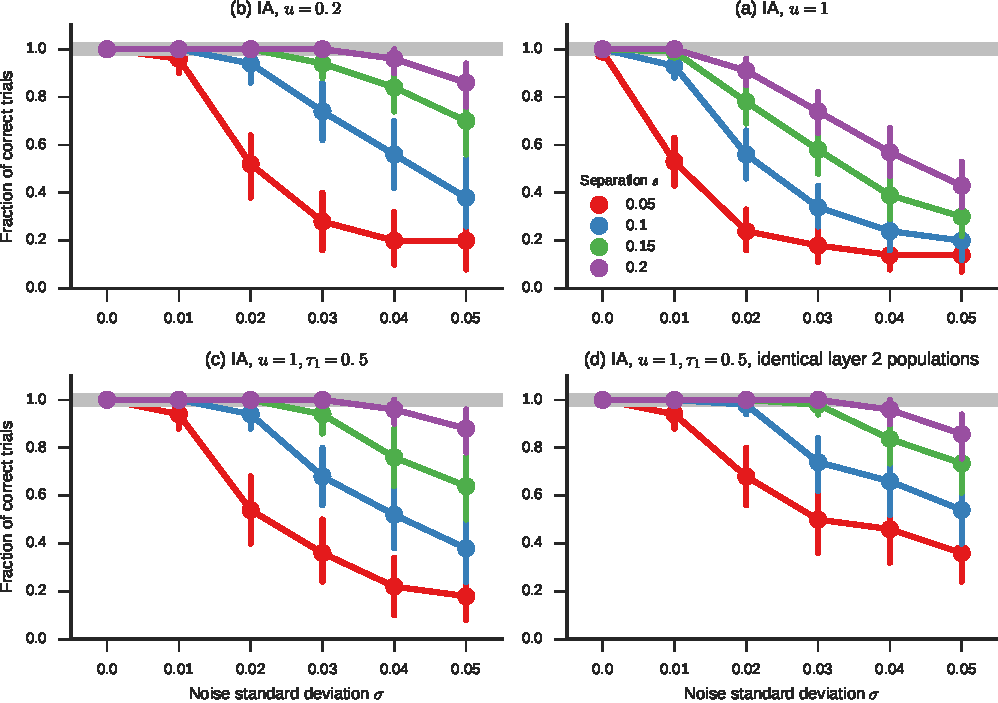
\includegraphics{figures/correct}
    \caption{
        Fraction of correct trials for different input noise standard deviations $\sigma$, target separations $s$, and models.  
        Error bars denote bootstrapped 95\% confidence intervals.
        The grey horizontal line shows the optimum.
    }\label{fig:correct}
\end{figure*}

The time required to reach a decision in the LCA network depends mostly on the target separation and the amount of noise on the input (see Fig.~\ref{fig:time}\todo{put a and b here too and reference them in the discussion}), the magnitude of the largest input is of minor influence.
Also, the confidence intervals indicate a larger variance in the decision times with less target separation and more input noise.
In contrast to that, in the IA network the scaled magnitude of the largest input is the most important factor.
Depending on this magnitude the network can either be faster or slower than the LCA network, but it will need more time to achieve the same fraction of correct responses.
There is also a slight influence of target separation and input noise with an interaction of these two parameters.
\begin{figure*}
    \centering
    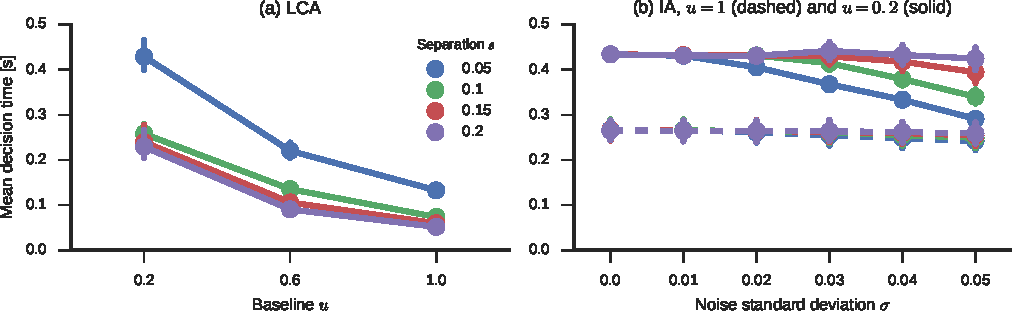
\includegraphics{figures/time}
    \caption{
        Mean decision times for different input noise standard deviations $\sigma$ and target separations $s$ for the LCA and IA networks.
        For the IA network $u = 0.2$ is shown which shows the interaction of target separation and input noise most clearly.
        Error bars denote bootstrapped 95\% confidence intervals.
        The grey horizontal lines show the optimum.
    }\label{fig:time}
\end{figure*}

The output of the IA network matches almost perfectly the specifications of producing an output of one for the winner and zero for all other choices \todo{a line on the LCA graph would help here too}.
This is not the case for the LCA network (see Fig.~\ref{fig:error}\todo{again a and b}).
For small target separations, the output of the winner will stay below $u$ and this will get worse with increased noise.
Furthermore, the LCA network will have residual outputs of losing choices under noisy conditions and with small target separations.
\begin{figure*}
    \centering
    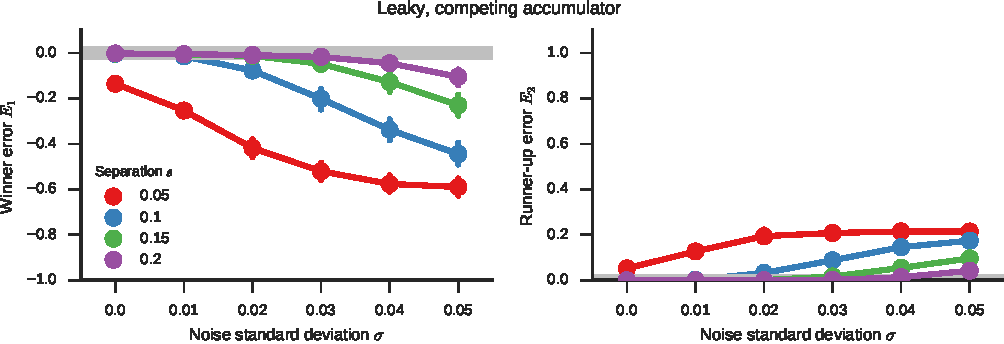
\includegraphics{figures/error}
    \caption{
        Error on outputs for different input noise standard deviations $\sigma$ and target separations $s$ for the LCA network.
        Error bars denote bootstrapped 95\% confidence intervals.
        The grey horizontal lines show the optimum.
    }\label{fig:error}
\end{figure*}

Finally, looking at the transient responses both models might produce outputs of losing choices (see Fig.~\ref{fig:transient}).
For the LCA network these increase with noise on the input and, for small target separation, can approach the final output of the winning choices.
For the IA network, transient outputs are smaller in noisy conditions, but can be higher than for the LCA network in less noisy conditions.
The magnitude of such transient responses is reduced by decreasing the input scaling.
\begin{figure*}
    \centering
    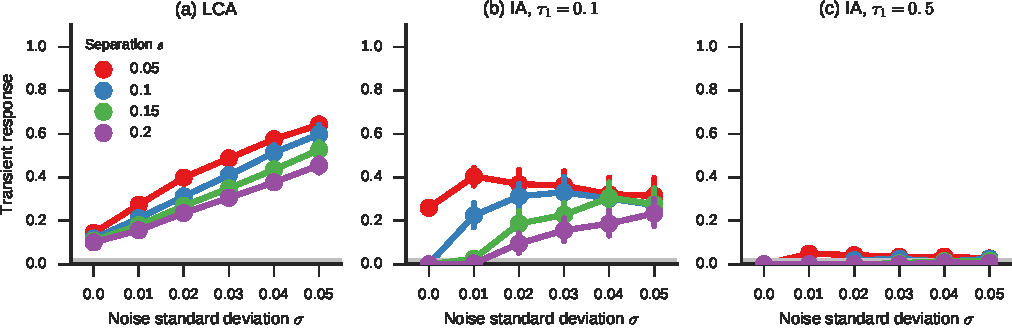
\includegraphics{figures/transient}
    \caption{
        Highest output of losing choices for different input noise standard deviations $\sigma$ and target separations $s$ for the LCA and IA networks.
        Error bars denote bootstrapped 95\% confidence intervals.
        The grey horizontal lines show the optimum.
    }\label{fig:transient}
\end{figure*}

\section{Discussion}
We have shown that neither network performs better on all benchmarks, but rather each is better suited for different purposes.
For instance, the LCA network determines the correct winner more quickly.
However, under noisy conditions it may not produce a clear output at all, and thus fails to make a decision.
The IA network might not be as quick or find the correct winner as often, but given enough time it will eventually arrive at a decision and produce a clear output.

Furthermore, the LCA network is especially well-suited for situations where a decision needs to be continuously adjusted.
The prescribed dynamics essentially try to output whatever the currently largest input is, while performing some smoothing over time.
This makes it quick to respond to changes in the input, but can also lead to randomly switching outputs due to noise.

In contrast, the IA network is better suited for situations where a discrete sequence of decisions is required.
After selecting a winner, the model's decision will persist due to self-excitation, even in the absence of input.
Thus, after making a decision, it is necessary to reset the model by inhibiting the winning accumulator.
This limits how quickly successive decisions can be made.
On the other hand, once a decision is made, the network provides a stable output.

When integrating these networks into larger neural or cognitive models, the two models present different challenges.
This integration is simpler for the IA network because the IA network provides a clear output.
The output of the winning choice is also always close to one, independent of the input, which makes it easy to detect when the decision has been made and processing can continue.
In contrast, detecting a decision is more problematic in the LCA network, where  a fluctuating output is often generated before the final decision, and the magnitude of the output depends on the input magnitude.
This makes it problematic to use a fixed threshold to detect the decision.
Furthermore, transient responses of losing choices can get close to the final output of the winning choice in the LCA network, making detection more difficult.

Part of the reason why the IA network produces less correct responses is the systematic bias introduced in the second layer.
By eliminating this bias through identical ensembles the correctness of the model is increased considerably.
However, this would require a very precise tuning of the neurons that might not be biologically plausible.

One critique of non-leaky accumulator models is that their ability to discriminate the largest input increases indefinitely with time \todo{~ref} and that there is no sensible stopping criterion.
However, this assumes that the time to reach a decision has no cost.
If time-to-decision has a cost, it will at some point exceed the gain achieved from making a correct decision.
Furthermore, this argument assumes integration with perfect accuracy.
But in a neural network resources are limited. As such the range and accuracy of values that can be represented in a neural population is limited.
At some point this would counterbalance any additional evidence.

We did not investigate the biological plausibility of these mechanisms in detail because this has been done before for different WTA networks \todo{ref???}.
Also, the implementation in spiking neurons ensures a certain level of biological plausibility.
We also did not look at at the influence of the number of dimensions $D$ in detail, but qualitatively the results will stay the same.
For higher $D$, we expect less accuracy since each additional choice has a baseline chance to win due to noise.
\todo{looking only at cases where a decision could be made within the results, include a number of parameters and github url}

\section{Notes}
Source code and supplementary analysis is available at \url{https://github.com/ctn-waterloo/cogsci17-decide}.
%These have not been peer reviewed.

\section{Acknowledgments}
This work was supported by the Canada Research Chairs program,
the NSERC Discovery grant 261453, Air Force Office of Scientific Research grant FA8655-13-1-3084, CFI, OIT, and NSERC CGS-D\@.  % chktex 8

\bibliographystyle{apacite}

\setlength{\bibleftmargin}{.125in}
\setlength{\bibindent}{-\bibleftmargin}

\bibliography{references}


\end{document} % chktex 17
